\clearpage
\cleardoublepage

\chapter{Dataset Processing}

\section{Data Collection}

The foundation of any machine learning system is quality data.

\subsection{Data Sources}

\begin{itemize}
    \item \textbf{Public datasets:} ImageNet, COCO, MNIST, etc.
    \item \textbf{Web scraping:} Automated data collection from websites
    \item \textbf{Sensors:} Cameras, microphones, medical devices
    \item \textbf{Human annotation:} Expert labeling
    \item \textbf{Synthetic data:} Generated from simulations
\end{itemize}

\begin{note}[Data Quality]
Garbage in, garbage out. High-quality data is more important than sophisticated algorithms.
\end{note}

\section{Data Annotation}

Labels enable supervised learning.

\subsection{Annotation Types}

\begin{itemize}
    \item \textbf{Classification:} Single label per image (cat vs dog)
    \item \textbf{Multi-label:} Multiple labels per image
    \item \textbf{Object detection:} Bounding boxes with labels
    \item \textbf{Semantic segmentation:} Pixel-wise labels
    \item \textbf{Instance segmentation:} Instance IDs per object
    \item \textbf{Keypoints:} Points of interest (faces, poses)
\end{itemize}

\begin{figure}[h]
    \centering
    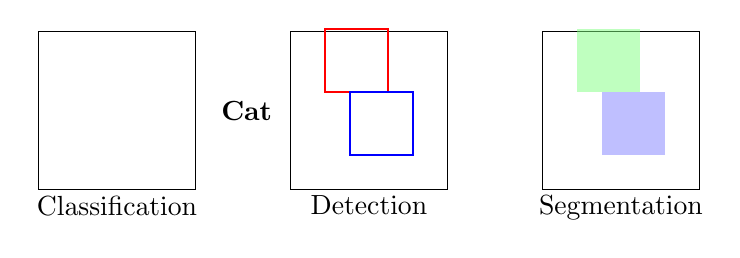
\begin{tikzpicture}[scale=0.8]
        % Classification
        \node[draw, rectangle, minimum width=2cm, minimum height=2cm] (cls) at (0,0) {};
        \node[below] at (0, -1.2) {Classification};
        \node[right] at (1.5, 0) {\textbf{Cat}};
        
        % Detection
        \node[draw, rectangle, minimum width=2cm, minimum height=2cm] (det) at (4,0) {};
        \draw[red, thick] (3.3, 0.3) rectangle (4.3, 1.3);
        \draw[blue, thick] (3.7, -0.7) rectangle (4.7, 0.3);
        \node[below] at (4, -1.2) {Detection};
        
        % Segmentation
        \node[draw, rectangle, minimum width=2cm, minimum height=2cm] (seg) at (8,0) {};
        \fill[green!50, opacity=0.5] (7.3, 0.3) rectangle (8.3, 1.3);
        \fill[blue!50, opacity=0.5] (7.7, -0.7) rectangle (8.7, 0.3);
        \node[below] at (8, -1.2) {Segmentation};
    \end{tikzpicture}
    \caption{Annotation types}
    \label{fig:annotation_types}
\end{figure}

\subsection{Annotation Tools}

\begin{itemize}
    \item \textbf{LabelImg:} Object detection bounding boxes
    \item \textbf{CVAT:} Computer Vision Annotation Tool
    \item \textbf{Supervisely:} Full-featured annotation platform
    \item \textbf{Amazon Mechanical Turk:} Crowdsourced annotation
    \item \textbf{Label Studio:} Open-source annotation tool
\end{itemize}

\section{Data Splitting}

Proper data splitting is crucial for unbiased evaluation.

\subsection{Basic Splits}

\begin{itemize}
    \item \textbf{Training set:} Used for model training
    \item \textbf{Validation set:} Used for hyperparameter tuning
    \item \textbf{Test set:} Used for final evaluation (only once)
\end{itemize}

Typical ratios:
\begin{itemize}
    \item Small datasets (<10K): 70/10/20 or 80/10/10
    \item Large datasets (>1M): 98/1/1 may suffice
\end{itemize}

\begin{note}[Test Set Leakage]
Never use test set for any decisions during training. This leads to overfitting to the test set and unreliable performance estimates.
\end{note}

\subsection{Stratified Splitting}

Maintains class distribution in each split:
\begin{verbatim}
from sklearn.model_selection import train_test_split
X_train, X_test, y_train, y_test = train_test_split(
    X, y, test_size=0.2, stratify=y
)
\end{verbatim}

\subsection{Cross-Validation}

For robust evaluation with limited data:

\begin{algorithm}[H]
\caption{K-Fold Cross-Validation}
\begin{enumerate}
    \item Split data into K folds
    \item For each fold:
    \begin{enumerate}
        \item Train on K-1 folds
        \item Validate on remaining fold
    \end{enumerate}
    \item Average performance across folds
\end{enumerate}
\end{algorithm}

Common values: K = 5 or 10

\section{Data Augmentation}

Artificially increase dataset size by transforming existing data.

\subsection{Image Augmentations}

\begin{itemize}
    \item \textbf{Rotation:} Random angle rotation
    \item \textbf{Flip:} Horizontal/vertical flips
    \item \textbf{Crop:} Random crops
    \item \textbf{Color jitter:} Brightness, contrast, saturation
    \item \textbf{Scale:} Random scaling
    \item \textbf{Translation:} Random shifts
    \item \textbf{Noise:} Gaussian noise injection
    \item \textbf{Cutout:} Random rectangular masking
    \item \textbf{Mixup:} Blend two images and labels
    \item \textbf{CutMix:} Cut and paste patches between images
\end{itemize}

\begin{code}
    \captionof{listing}{Data Augmentation in PyTorch}
    \label{code:augmentation}
\begin{lstlisting}[language=python]
import torchvision.transforms as T

train_transform = T.Compose([
    T.RandomResizedCrop(224),
    T.RandomHorizontalFlip(p=0.5),
    T.RandomRotation(15),
    T.ColorJitter(brightness=0.2, contrast=0.2, 
                  saturation=0.2, hue=0.1),
    T.ToTensor(),
    T.Normalize(mean=[0.485, 0.456, 0.406],
                std=[0.229, 0.224, 0.225])
])

val_transform = T.Compose([
    T.Resize(256),
    T.CenterCrop(224),
    T.ToTensor(),
    T.Normalize(mean=[0.485, 0.456, 0.406],
                std=[0.229, 0.224, 0.225])
])
\end{lstlisting}
\end{code}

\begin{figure}[h]
    \centering
    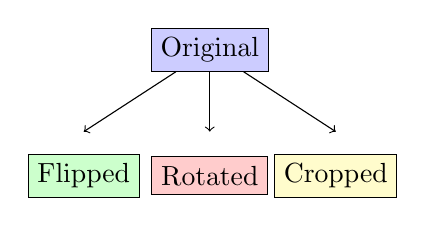
\begin{tikzpicture}[scale=0.8]
        % Original
        \node[draw, rectangle, fill=blue!20] (orig) at (0,0) {Original};
        
        % Augmentations
        \node[draw, rectangle, fill=green!20] at (-2, -2) {Flipped};
        \node[draw, rectangle, fill=red!20] at (0, -2) {Rotated};
        \node[draw, rectangle, fill=yellow!20] at (2, -2) {Cropped};
        
        % Arrows
        \draw[->] (orig) -- (-2, -1.3);
        \draw[->] (orig) -- (0, -1.3);
        \draw[->] (orig) -- (2, -1.3);
    \end{tikzpicture}
    \caption{Data augmentation examples}
    \label{fig:augmentation}
\end{figure}

\subsection{Advanced Augmentation}

\begin{itemize}
    \item \textbf{AutoAugment:} Learned augmentation policies
    \item \textbf{RandAugment:} Simpler policy search
    \item \textbf{TrivialAugment Wide:} No search needed
    \item \textbf{Test-Time Augmentation (TTA):} Augment at test time, average predictions
\end{itemize}

\section{Data Loading}

Efficient data loading is crucial for training speed.

\begin{code}
    \captionof{listing}{Data Loading in PyTorch}
    \label{code:dataloader}
\begin{lstlisting}[language=python]
from torch.utils.data import DataLoader, Dataset

class MyDataset(Dataset):
    def __init__(self, data, labels, transform=None):
        self.data = data
        self.labels = labels
        self.transform = transform
    
    def __len__(self):
        return len(self.data)
    
    def __getitem__(self, idx):
        image = self.data[idx]
        label = self.labels[idx]
        
        if self.transform:
            image = self.transform(image)
        
        return image, label

# Create dataloaders
train_loader = DataLoader(
    train_dataset,
    batch_size=32,
    shuffle=True,  # Important for SGD
    num_workers=4,  # Parallel data loading
    pin_memory=True,  # Faster GPU transfer
    drop_last=True  # Consistent batch sizes
)

# Iterate
for batch_idx, (images, labels) in enumerate(train_loader):
    # images: (B, C, H, W)
    # labels: (B,)
    pass
\end{lstlisting}
\end{code}

\begin{properties}[DataLoader Best Practices]
\begin{itemize}
    \item Use multiple workers for parallel loading
    \item Enable pin\_memory for faster GPU transfer
    \item Set shuffle=True for training
    \item Consider drop\_last for consistent batch sizes
\end{itemize}
\end{properties}

\section{Normalization}

Standardize input features for better training.

\subsection{Image Normalization}

\begin{equation}
x_{norm} = \frac{x - \mu}{\sigma}
\end{equation}

Common ImageNet normalization:
\begin{itemize}
    \item Mean: $[0.485, 0.456, 0.406]$
    \item Std: $[0.229, 0.224, 0.225]$
\end{itemize}

Compute dataset-specific normalization:
\begin{lstlisting}[language=python]
# Compute mean and std
loader = DataLoader(dataset, batch_size=32)
mean = 0.0
std = 0.0
for images, _ in loader:
    batch_samples = images.size(0)
    images = images.view(batch_samples, images.size(1), -1)
    mean += images.mean(2).sum(0)
    std += images.std(2).sum(0)
mean /= len(loader.dataset)
std /= len(loader.dataset)
\end{lstlisting}

\section{Chapter Summary}

\begin{enumerate}
    \item Data quality is fundamental to model performance
    \item Annotation types depend on the task
    \item Proper data splitting prevents overfitting
    \item Data augmentation improves generalization
    \item Efficient data loading accelerates training
    \item Normalization stabilizes training
\end{enumerate}
